\usetikzlibrary{decorations.pathreplacing}
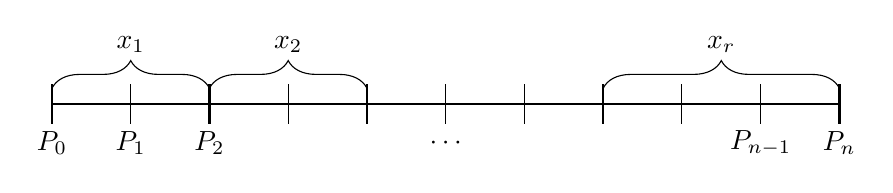
\begin{tikzpicture}
\draw[thick] (0,0)--(10,0);

\draw[thick] (0,-0.25)--(0,0.25);
\draw (1,-0.25)--(1,0.25);
\draw[thick] (2,-0.25)--(2,0.25);
\draw (3,-0.25)--(3,0.25);
\draw[thick] (4,-0.25)--(4,0.25);
\draw (5,-0.25)--(5,0.25);
\draw (6,-0.25)--(6,0.25);
\draw[thick] (7,-0.25)--(7,0.25);
\draw (8,-0.25)--(8,0.25);
\draw (9,-0.25)--(9,0.25);
\draw[thick] (10,-0.25)--(10,0.25);


\draw [decorate, decoration={brace, amplitude=10pt}] (0,0.2)--(2,0.2);
\node at (1,0.75) {$x_1$};

\draw [decorate, decoration={brace, amplitude=10pt}] (2,0.2)--(4,0.2);
\node at (3,0.75) {$x_2$};

\draw [decorate, decoration={brace, amplitude=10pt}] (7,0.2)--(10,0.2);
\node at (8.5,0.75) {$x_r$};

\node at (0,-0.5) {$P_0$};
\node at (1,-0.5) {$P_1$};
\node at (2,-0.5) {$P_2$};
\node at (9,-0.5) {$P_{n-1}$};
\node at (10,-0.5) {$P_n$};
\node at (5,-0.5) {$\cdots$};

\end{tikzpicture}